\chapter{Evaluation}
\label{cha:evaluation}
\begin{figure}[ht]
    \centering
    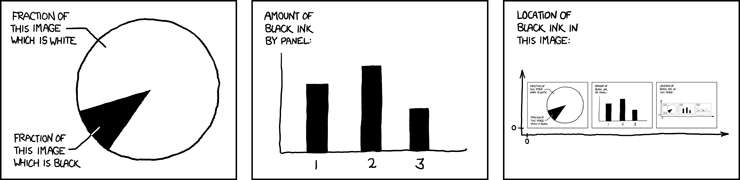
\includegraphics[width=\textwidth]{xkcd/688.png}
    \caption*{Source: \href{https://xkcd.com/688/}{xkcd}}
\end{figure}


some kind of introduction

%=min(A2,C2,E2,G2,I2,K2,M2,O2,Q2,S2,U2)

\section{Baseline experiment}    
The first experiments consists of the stable network with 10 Binge persona client added afterwards, with a uniform randomized delay before they start between 0 and 60 seconds. The bandwidth for the clients is set at 20 \acs{MBit} and no artificial latency is added. The network used is closed meaning only the relevant peers are present. It is expected to perform well with almost no stalls or failures, and segments are expected to be retrieved with low latency. Clients are expected to download about 56 \acs{MB} which is the size of the video, which is 90 seconds long. \\
In the experiment every client stalled exactly once (See figure \ref{plot:baseline_stall_time}), which happened when the video was being initially started and the buffer was getting filled, this can therefore not be considered a failure, meaning the users got a good quality of experience.\\ 

\begin{figure}[ht]
    \myfloatalign
    \begin{tikzpicture}
        \begin{axis} [
            xlabel={Experiment Time (seconds)},
            ylabel={Accumulated stall time (\acs{ms})},
            x filter/.code={\pgfmathparse{#1/1000}\pgfmathresult},
            ]
            \addplot[
            unbounded coords=jump,
            sharp plot] table[
            x=x1,
            y=y1
            ]{./data/baseline/stall_time.csv};
            \addplot[
            unbounded coords=jump,
            sharp plot] table[
            x=x2,
            y=y2
            ]{./data/baseline/stall_time.csv};
            \addplot[
            unbounded coords=jump,
            sharp plot] table[
            x=x3,
            y=y3
            ]{./data/baseline/stall_time.csv};
            \addplot[
            unbounded coords=jump,
            sharp plot] table[
            x=x4,
            y=y4
            ]{./data/baseline/stall_time.csv};
            \addplot[
            unbounded coords=jump,
            sharp plot] table[
            x=x5,
            y=y5
            ]{./data/baseline/stall_time.csv};
            \addplot[
            unbounded coords=jump,
            sharp plot] table[
            x=x6,
            y=y6
            ]{./data/baseline/stall_time.csv};
            \addplot[
            unbounded coords=jump,
            sharp plot] table[
            x=x7,
            y=y7
            ]{./data/baseline/stall_time.csv};
            \addplot[
            unbounded coords=jump,
            sharp plot] table[
            x=x8,
            y=y8
            ]{./data/baseline/stall_time.csv};
            \addplot[
            unbounded coords=jump,
            sharp plot] table[
            x=x9,
            y=y9
            ]{./data/baseline/stall_time.csv};
            \addplot[
            unbounded coords=jump,
            sharp plot] table[
            x=x10,
            y=y10
            ]{./data/baseline/stall_time.csv};
        \end{axis}
    \end{tikzpicture}
    \caption[Stalls over time from baseline exp.]{Stalls over time from the baseline experiment. The users stall at the beginning and afterwards not at all, signifying a good user experience.}
    \label{plot:baseline_stall_time}
\end{figure}


In terms of amount of data received on the clients, a single peer downloaded about the expected amount, and every other peer downloaded more and more. In the worst case about 7 times more (See figure \ref{plot:baseline_network_rx_bytes_time}).

\begin{figure}[ht]
    \myfloatalign
    \begin{tikzpicture}
    \begin{axis}[
        ybar,
        ymin=0,
        bar width = 4pt,
        y filter/.code={\pgfmathparse{#1/1024^2}\pgfmathresult},
        xtick=data,
        xticklabels from table={./data/baseline/network_hist.csv}{users},
        x tick label style={rotate=60, anchor=east},
        ylabel={Accumulated bandwidth (\acs{MB})},
        legend style={at={(1.05,1)}, anchor=north west,legend columns=1},]
        \addplot table [
            x expr=\coordindex,
            y={rx},
            ]{./data/baseline/network_hist.csv};
        \addplot table [x expr=\coordindex, y={tx}]{./data/baseline/network_hist.csv};
        \addplot[black, sharp plot, update limits=false]
                coordinates{(-1, 55992320) (11, 55992320)};
        \legend{received,transmitted}
    \end{axis}
    \draw (8,0.75) node {video size};
    \end{tikzpicture}
    \caption[Total bandwidth from baseline exp.]{Recieved and transmitted bytes per client, from the baseline experiment. Download overhead is as large as factor 1:7 as exemplified by \textit{8:BINGE} recieving 389 \ac{MB} while asking for a 56 \acs{MB} video.}
    \label{bar:baseline_network_hist}
\end{figure}


Since the video segments are the only files being distributed in the network the extra data being downloaded must be duplicate data. We can also observe that the ones downloading the least are also the clients that get to watch the video first, where the files are least distributed.\\ 

\begin{figure}[ht]
    \myfloatalign
    \begin{tikzpicture}
        \begin{axis} [
            xlabel={Experiment Time (seconds)},
            ylabel={Recieved data (\acs{MB})},
            legend style={at={(1.05,1)}, anchor=north west,legend columns=1},
            y filter/.code={\pgfmathparse{#1/1024^2}\pgfmathresult},
            ]
            \addplot[color=red,
            unbounded coords=jump,
            sharp plot] table[
            x=x1,
            y=y1
            ]{./data/baseline/network_rx_bytes_time.csv};
            \addplot[
            unbounded coords=jump,
            sharp plot] table[
            x=x2,
            y=y2
            ]{./data/baseline/network_rx_bytes_time.csv};
            \addplot[
            unbounded coords=jump,
            sharp plot] table[
            x=x3,
            y=y3
            ]{./data/baseline/network_rx_bytes_time.csv};
            \addplot[
            unbounded coords=jump,
            sharp plot] table[
            x=x4,
            y=y4
            ]{./data/baseline/network_rx_bytes_time.csv};
            \addplot[
            unbounded coords=jump,
            sharp plot] table[
            x=x5,
            y=y5
            ]{./data/baseline/network_rx_bytes_time.csv};
            \addplot[
            unbounded coords=jump,
            sharp plot] table[
            x=x6,
            y=y6
            ]{./data/baseline/network_rx_bytes_time.csv};
            \addplot[
            unbounded coords=jump,
            sharp plot] table[
            x=x7,
            y=y7
            ]{./data/baseline/network_rx_bytes_time.csv};
            \addplot[
            unbounded coords=jump,
            sharp plot] table[
            x=x8,
            y=y8
            ]{./data/baseline/network_rx_bytes_time.csv};
            \addplot[
            unbounded coords=jump,
            sharp plot] table[
            x=x9,
            y=y9
            ]{./data/baseline/network_rx_bytes_time.csv};
            \addplot[
            unbounded coords=jump,
            sharp plot] table[
            x=x10,
            y=y10
            ]{./data/baseline/network_rx_bytes_time.csv};
            \legend{1:BINGE,2-10:BINGE}
        \end{axis}
    \end{tikzpicture}
    \caption[Recieved data from baseline exp.]{Recieved data over time from the baseline experiment.}
    \label{plot:baseline_network_rx_bytes_time}
\end{figure}


In terms of latency in acquiring the files, it is varies greatly between each segment and no pattern can be observed, but for the average latency of every client the best performing client has an average of 1053\acs{ms} and the worst has an average of 912\acs{ms}. \begin{table}[ht]
    \caption[Mean of latencies from baseline exp.]{Mean of latencies of segment downloads per client, from the baseline experiment (\expid{B10}). Measured across 30 segments. Clients that started later have lower latency, although not by much.}
    \label{tab:binge_latency_mean}
    \myfloatalign
    \pgfplotstabletypeset[
        every head row/.style={
            before row=\toprule,
            after row=\midrule,
        },
        every even row/.style={
            before row={\rowcolor{gray!10}}
        },
        every last row/.style={
            after row=\bottomrule
        },
        columns={user,latency},
        columns/user/.style={
            column name={Clients},
            string type,
        },
        columns/latency/.style={
            column name={Latency (\acs{ms})},
            column type = r,
        },
    ]{./data/baseline/video_latency_mean_seg.csv}
\end{table}
So even though the worst performing downloads 7 times the data it does not seem to impact it negatively, this might change however as it is expected that the network could get flooded if this factor increases more with even more peers.

\subsection{Smaller network experiments}
The baseline experiment is also repeated with smaller amounts of Binge users in the network, this is primarily used for comparison in the future experiments.

\section{Leecher population experiment}
In this experiment we alter the percentage of leechers versus bingers that the network contains, otherwise the conditions are the same as the baseline experiment.
Based on the first experiment adding leechers to the network should decrease the amount of duplicate data being sent, but it also means more requests to the holders of the video segments potentially as there is fewer sources to get them from. Therefore the network is expected to perform better as long as the Seeder can keep up.\\
The results however were different from expected, having a single leecher in the network, had no real impact on the bingers, but the leecher user got very high stall time, over 17 seconds with stalls spread across the video rather than just at the beginning. 

%stall_time and stall_time_hist (/home/kgoyo/cs_project/home/auuser/flixtube/data/plot/2018-05-15_16:21:32.688486)

\begin{figure}[ht]
    \myfloatalign
    \begin{tikzpicture}
        \begin{axis} [
            xlabel={Experiment Time (seconds)},
            ylabel={Stall time (seconds)},
            legend style={at={(1.05,1)}, anchor=north west,legend columns=1},
            x filter/.code={\pgfmathparse{#1/1000}\pgfmathresult},
            y filter/.code={\pgfmathparse{#1/1000}\pgfmathresult},
            ]
            \addplot[
            unbounded coords=jump,
            sharp plot] table[
            x=x1,
            y=y1
            ]{./data/leecher/stall_time_leecher.csv};
            \addplot[
            color=red,
            unbounded coords=jump,
            sharp plot] table[
            x=x10,
            y=y10
            ]{./data/leecher/stall_time_leecher.csv};
            \addplot[
            unbounded coords=jump,
            sharp plot] table[
            x=x2,
            y=y2
            ]{./data/leecher/stall_time_leecher.csv};
            \addplot[
            unbounded coords=jump,
            sharp plot] table[
            x=x3,
            y=y3
            ]{./data/leecher/stall_time_leecher.csv};
            \addplot[
            unbounded coords=jump,
            sharp plot] table[
            x=x4,
            y=y4
            ]{./data/leecher/stall_time_leecher.csv};
            \addplot[
            unbounded coords=jump,
            sharp plot] table[
            x=x5,
            y=y5
            ]{./data/leecher/stall_time_leecher.csv};
            \addplot[
            unbounded coords=jump,
            sharp plot] table[
            x=x6,
            y=y6
            ]{./data/leecher/stall_time_leecher.csv};
            \addplot[
            unbounded coords=jump,
            sharp plot] table[
            x=x7,
            y=y7
            ]{./data/leecher/stall_time_leecher.csv};
            \addplot[
            unbounded coords=jump,
            sharp plot] table[
            x=x8,
            y=y8
            ]{./data/leecher/stall_time_leecher.csv};
            \addplot[
            unbounded coords=jump,
            sharp plot] table[
            x=x9,
            y=y9
            ]{./data/leecher/stall_time_leecher.csv};
            \legend{1-9:BINGE,10:LEECHER}
        \end{axis}
    \end{tikzpicture}
    \caption[Stalls over time from 1 Leecher exp.]{Stalls over time from the 1 Leecher experiment. The leecher stalls multiple times during the experiment and not only at the beginning like the binge users.}
    \label{plot:leecher_stall_time}
\end{figure}


\begin{figure}[ht]
    \myfloatalign
    \begin{tikzpicture}
    \begin{axis}[
        ybar,
        ymin=0,
        y filter/.code={\pgfmathparse{#1/1000}\pgfmathresult},
        xtick=data,
        xticklabels from table={./data/leecher/stall_time_hist_leecher.csv}{users},
        x tick label style={rotate=60, anchor=east},
        ylabel=\shortstack{Accumulated stall time\\(seconds)},
        legend style={at={(1.05,1)}, anchor=north west,legend columns=1},]
        \addplot table [x expr=\coordindex, y={rx}]{./data/leecher/stall_time_hist_leecher.csv};
    \end{axis}

    \end{tikzpicture}
    \caption[Total stall time from \expid{L1B9}]{Total stall time per client, from the 1 Leecher and 9 Binge experiment (\expid{L1B9}).\\Only the leecher stalls for a long time, while binge users barely stall at all.}
    \label{bar:leecher_stall_time_hist}
\end{figure}


Scaling the network to having half of the users being leechers and the other half bingers, negatively impacted all the clients, as the 5 bingers now had an average stall time of about 13 seconds while the stall time for the leechers became much worse with an average of about 53 seconds. For both types of clients the standard deviation of stall time was around 10 seconds, meaning the users got vastly different performances, and even two of the binger only stall once at the beginning of the video, meaning they got a good quality of experience.

%stall_hist, stall_hist_role_mean and stall_hist_role_stdev (/home/kgoyo/cs_project/home/auuser/flixtube/data/plot/2018-05-15_15:51:32.232356)

\begin{figure}[ht]
    \myfloatalign
    \begin{tikzpicture}
    \begin{axis}[
        ybar,
        ymin=0,
%        bar width = 4pt,
        xtick=data,
        xticklabels from table={./data/leecher/stall_hist_leecher.csv}{users},
        x tick label style={rotate=60, anchor=east},
        ylabel={\# Stalls},
        legend style={at={(1.05,1)}, anchor=north west,legend columns=1},]
        \addplot table [x expr=\coordindex, y={stalls}]{./data/leecher/stall_hist_leecher.csv};
    \end{axis}

    \end{tikzpicture}
    \caption[Total number stalls from 1 Leecher exp.]{Total number of stalls per client, from the 5 Leecher experiment}
    \label{bar:leecher_stall_hist}
\end{figure}

\begin{figure}[ht]
    \myfloatalign
    \begin{tikzpicture}
    \begin{axis}[
            ybar,
            ymin=0,
            bar width=0.35,
            enlarge x limits={abs=0.4},
            xtick=data,
            xticklabels from table={./data/leecher/stall_hist_role_leecher.csv}{users},
            ylabel={Mean accumulated stall time (\acs{s})},
            legend style={at={(1.05,1)}, anchor=north west,legend columns=1},
        ]

        \addplot[
            fill=blue!30,
            draw=blue,
            error bars,
            y dir=both,
            y explicit,
            error bar style={red},
        ] 
        table [
            x expr=\coordindex,
            y expr=\thisrow{mean}/1000,
            y error expr=\thisrow{stddev}/1000
        ]{./data/leecher/stall_hist_role_leecher.csv};
        
    \end{axis}

    \end{tikzpicture}
    \caption[Stall time per client from \expid*{L5B5} and \expid*{L10}]{Mean of the accumulated stall time for each type of client for: \\ 
    {[1]} is a network with 5 Leechers and 5 Bingers (\expid{L5B5}, \\ 
    {[2]} is a network with 10 Leechers (\expid{L10}).\\
    Adding more Leechers gives more stall time for each Leecher, while Bingers are less affected.}
    \label{bar:leecher_stall_hist_role}
\end{figure}


%stall_time and stall_time_hist_role_mean (/home/kgoyo/cs_project/home/auuser/flixtube/data/plot/2018-05-15_16:41:32.810778)
% added in data/leecher/stall_hist_role_leecher.tex and the stall_time_hist below instead of stall_time
%\begin{figure}[ht]
    \myfloatalign
    \begin{tikzpicture}
    \begin{axis}[
        ybar,
        ymin=0,
%        bar width = 4pt,
        xtick=data,
        xticklabels from table={./data/leecher/stall_time_hist_leecher10.csv}{users},
        x tick label style={rotate=60, anchor=east},
        ylabel=Total stall time (ms),
        legend style={at={(1.05,1)}, anchor=north west,legend columns=1},]
        \addplot table [x expr=\coordindex, y={rx}]{./data/leecher/stall_time_hist_leecher10.csv};
    \end{axis}

    \end{tikzpicture}
    \caption{Total stall time per client, from the 10 leechers experiment}
    \label{bar:leecher_stall_time_hist}
\end{figure}


Scaling the amount of leechers further, to all the clients being leechers, increased the bad quality of experience further, and the total mean stall time became 100 seconds, that occured frequently during the video.

These results show that leeching off of a public \acs{IPFS} gateway is punished compared to the users retrieving the files themselves and using their own gateway. And the tit-for-tat principle is enforced. Unfortunately leechers still impacted the well behaving binge users's quality of experience as they experience more stalling as the percentage of leechers in the network grew.\\
In terms of data downloaded leecher users were much more efficient, in the half binger half leecher experiment. The leechers only downloaded on average about 60\acs{MB} which is only slightly higher than the file size of the video files. While the bingers on average downloaded about 140\acs{MB}, which is more than double of what the leechers did. 
\begin{figure}[ht]
    \myfloatalign
    \begin{tikzpicture}
    \begin{axis}[
        ybar,
        ymin=0,
        y filter/.code={\pgfmathparse{#1/1024^2}\pgfmathresult},
        bar width=0.3,
        enlarge x limits={abs=0.4},
        xtick=data,
        xticklabels from table={./data/leecher/network_hist_comparison.csv}{users},
%        x tick label style={rotate=60, anchor=east},
        ylabel=Mean accumulated bandwidth (\acs{MB}),
        legend style={at={(1.05,1)}, anchor=north west,legend columns=1},]
        \addplot 
            table [
                x expr=\coordindex,
                y={rx},
            ]{./data/leecher/network_hist_comparison.csv};
        \addlegendentry{received}
        
        \addplot
            table [
                x expr=\coordindex,
                y={tx},
            ]{./data/leecher/network_hist_comparison.csv};
        \addlegendentry{transmitted}
        
%        \addlegendimage{empty legend}
%        \addlegendimage{empty legend}
%        \addlegendentry{\hspace{-34pt}(1) \hspace{17pt} B5}
%        \addlegendentry{\hspace{-29pt}(2) \hspace{9pt} L5B5}
        
        \addplot [
                black, 
                sharp plot, 
                update limits=false
            ] coordinates{(-1, 55992320) (11, 55992320)};
    \end{axis}
    \draw (8,2) node {video size};
    \end{tikzpicture}
    \caption[Mean bandwidth per client comparison between \expid*{B5} and \expid*{L5B5}]{Comparison of the mean of accumulated bandwidth for each type of client for; \newline
     {[1]} a network with 5 Bingers (\expid{B5}), \newline
     {[2]} a network with 5 Leechers and 5 Bingers (\expid{L5B5}). \newline 
    Leechers are more efficient in the amount of data they download while Bingers downloads duplicate data. Bingers had very similar amount of received data regardless if there are Leechers present or not.}
    \label{bar:leecher_network_hist_comparison}
\end{figure}


Having a network of only 5 binger users in comparison gave an average of about 120\acs{MB} of downloaded data, as both cases had fairly high standard deviation this is within the margin of error. But adding leechers to the network does not seem to harm the binger users in terms of the amount of data they have to download but instead it might lower it as they get less access to the Seeder, meaning they have to rely on the other users more.

\section{Impact of skipper personas experiment}
This experiment has another client behaviour in the skipper persona, the goal is to see what kind of impact the skipper has on the network as a whole and if it can negatively impact a Binge user. We also want to see what kind of performance a skipper gets when watching a video, the video should stall every time the client skips in the video. But the amount of time spent in the stalling state should ideally be small, but based on the latency seen in the baseline experiment, it is likely that it stalls for more than a second after every skip as this is the latency seen when acquiring segments. The configuration of the skipper is to watch for 3 seconds and then skip ahead 10 seconds. If the only stalls are because of skips, they should have exactly 7 stalls each.
In the experiments skipper users got around 7 stalls, meaning they did not stall more than they were required to do by the persona behaviour, the amount of skippers in the network did not impact the amount of stalls. The time spent stalling is also unaffected as can be seen from the experiment with 5 skippers versus the one with 10. The average time spent stalling for skipper personas were about the same. %stall_hist_role_mean (/home/kgoyo/cs_project/home/auuser/flixtube/data/plot/2018-05-15_13:21:29.634478) (/home/kgoyo/cs_project/home/auuser/flixtube/data/plot/2018-05-15_13:41:31.386109)
The quality of experience for the binge users also seemed unaffected, as they like the baseline experiment still only stalled at the start, and infrequently once more after that. %stall_hist (/home/kgoyo/cs_project/home/auuser/flixtube/data/plot/2018-05-15_13:21:29.634478) (/home/kgoyo/cs_project/home/auuser/flixtube/data/plot/2018-05-15_12:51:31.043665)
Although the binge users did tend to download more data than the skippers, this can be excused to the skippers going ahead in progress in the video faster than the binge users. Meaning they will have the segments before and as the binge users reach that point in the video and requests segments relevant to it. Those segments are more duplicated in the network resulting in downloading more duplicates. %rx_bytes_tx_bytes_hist_role_mean (/home/kgoyo/cs_project/home/auuser/flixtube/data/plot/2018-05-15_13:21:29.634478)
The only thing that made skippers stand out in comparison to binge users is that when trying to retrieve segments, they got more errors. Errors meaning that the request returning a responsecode not corresponding to OK. Bingers almost never got errors but with skippers in the network a fair amount of segments had users get errors when trying to retrieve them. %TODO try to explain why this happens %failure_hist_video (/home/kgoyo/cs_project/home/auuser/flixtube/data/plot/2018-05-15_13:21:29.634478)
In conclusion skippers have very little impact in relation to the network and the worsened performance is isolated within themselves with little to no negative impact on the other users in the network.

\subsection{Skipper configurations}
The skipper can be configured in both the amount of time it watches videos in between skips, and how far forward it skips, which is tested in a single network configuration in this experiment. %todo decide on a configuration
The watch time is expected to have little impact as the dash player buffer should be about full at all times. But adjusting skipper length means that potentially more of the buffer has to be replaced and if the skipper length is set high enough. The entirety of the buffer is replaced. %todo find what is dash player buffer length

\section{Impact of incognito personas experiment}
This experiment has the incognito behaviour in the network, which is expected to only impact a small amount of segment of the video, the segments that are watched by the incognito users. For the rest of the segments we should see similar results to the baseline experiment with equal amount of binge users. Based on the experiments with the skipper user, the binge users are not expected to be affected by the incognito user in terms of quality of experience.\\
In the experiment incognito users performed like binge users that just watched a shorter video. They stalled exactly once like binge users, and users that watched segments late had to download more like binge users. %stall_hist and network_rx_bytes_tx_bytes_hist 
Unlike binge users the initial stall was much longer, in the 5 binge users and 5 incognito users experiment. Bingers stalled for an average about 0.4 seconds while incognito was at 2 seconds. This delay might be because of the incognito user initially downloads the first segments of the video and then skips to the end of the video and starts downloading new ones. The dash player also has to determine which segment correspond to the specific timestamp, which can add to the stalling time.
\begin{figure}[ht]
    \myfloatalign
    \begin{tikzpicture}
    \begin{axis}[
        ybar,
        ymin=0,
        bar width=0.75,
        enlarge x limits={abs=1},
        xtick=data,
        xticklabels from table={./data/incognito/stall_hist_role.csv}{users},
%        x tick label style={rotate=60, anchor=east},
        ylabel={Mean of accumulated stall time (\acs{ms})},
        legend style={at={(1.05,1)}, anchor=north west,legend columns=1},]
        \addplot table [x expr=\coordindex, y={time}]{./data/incognito/stall_hist_role.csv};
    \end{axis}

    \end{tikzpicture}
    \caption[Mean stall time from 5 Incognito exp.]{Mean of sccumulated stall time for Binge clients compared to Incognito clients, from the 5 Incognito experiment. \newline Incognito users stall much longer before they start playing the video.}
    \label{bar:incognito_stall_role}
\end{figure}

In terms of downloaded data the binge users had to download slightly more compared to the baseline experiments, for instance 5 binge users with 5 incognito users meant that the bingers downloaded on average 145\acs{MB}, compared to having 5 bingers alone downloading 84\acs{MB}. This can be explained by the later segments of the video being more available, leading to an increase in duplicate data, which is in line with the other results.
\begin{figure}[ht]
    \myfloatalign
    \begin{tikzpicture}
    \begin{axis}[
        ybar,
        ymin=0,
        y filter/.code={\pgfmathparse{#1/1024^2}\pgfmathresult},
        bar width=0.35,
        enlarge x limits={abs=0.75},
        xtick=data,
        xticklabels from table={./data/incognito/network_rx_bytes_tx_bytes_hist_role_mean.csv}{users},
        ylabel=Mean accumulated bandwidth (\acs{MB}),
        legend style={at={(1.05,1)}, anchor=north west,legend columns=1},]
        \addplot table [x expr=\coordindex, y={rx}]{./data/incognito/network_rx_bytes_tx_bytes_hist_role_mean.csv};
        \addplot table [x expr=\coordindex, y={tx}]{./data/incognito/network_rx_bytes_tx_bytes_hist_role_mean.csv};
        \legend{received,transmitted}
    \end{axis}

    \end{tikzpicture}
    \caption[Mean bandwidth of Binge with and without Incognito]{Mean of the accumulated data received and transmitted for 5 Binge with and without 5 Incognito users in the network (\expid{I5B5} and \expid{B5}). \newline With incognito users the amount downloaded data is increased by around 50\%.}
    \label{bar:incognito_hist_net}
\end{figure}


\section{Impact of idle users}
In this experiment we measure how adding a few idle users to the network affects bingers, this experiment functions as a smaller scale global \acs{IPFS} as the irrelevant peers in that network functions somewhat like the idle users in this test. It is expected that having idle users fill up the \acs{DHT}s on the binge user should increase the amount of latency in the network slightly. But otherwise it should stay about the same.

\section{Mobile users experiment}
This experiment in terms of behaviour is the same as the baseline, but the network conditions are worsened  in terms of the bandwidth available and/or latency. 

\subsection{Low bandwidth network}
In these experiments the amount of bandwidth available to the clients is decreased, this should punish \acs{IPFS} more for its excessive amount of data being transmitted between peers. 5MBit is chosen as a lower bound, as decreasing the bandwidth lower than this would result in not having enough for just watching the video alone from a single source, without any other network communication.
% low bandwidth (minimum theoretical is (56 /90 *8 = approx 5 MBit)

\subsection{High latency network}
High latency is expected to increase the amount of duplicate data the clients receive, as changed in the peers want list take longer to propogate to peers that have segments that are no longer wanted. It could potentially also increase the amount of stalls, since it takes too long for the relevant segments to arrive to the client that needs them.

\subsection{combination of the two previous networks}
This experiments combines the network configuration of the 2 previous experiments, to test how \acs{IPFS} performs under very bad conditions. % results are probably similar to the previous experiments

\subsection{Jittery network conditions}
In this experiment the conditions of a mobile users are emulated, where the conditions can sometimes be very good and sometimes become too bad to watch video for short amounts of time, where the buffer being filled should be able to keep the video running smoothly, as long as the conditions are not bad for too long.

\section{Leaver impact experiment}
The clients can also leave the network after they have finished watching the video, meaning they would no longer provide the video to other peers. The experiment is based on the baseline, but where clients leave when they are done. Based on the results of the baseline this should result in reduced duplicate data as the clients that join the network early, that also got less duplicates, leave before the other clients are done. And when they do that is one less duplicate that the other clients receive.

\section{Lower socialness impact experiment}
The other experiments are focused on having all clients watch the video at the same time with very little difference in when they start the video. This experiment increases the time between startup effectively lowering the socialness of the video, as it becomes less viral. Although to properly test the impact of socialness the experiments have to last much longer, multiple days, which is omitted and replaced with the smaller timeframe experiment instead.

\section{Global IPFS}
In the other experiments all clients in the \acs{IPFS} network were relevant to the video files, contrary to the intended design of \acs{IPFS} where all users of \acs{IPFS} are in a shared network regardless of the content they have. This experiment runs the same configuration as the baseline but in the global \acs{IPFS} instead, it is expected to perform similar to increasing the latency as having larger network means larger hash tables, which results in having longer lookup times for the video segments.

%%% Local Variables:
%%% mode: latex
%%% TeX-master: "../ClassicThesis"
%%% ispell-dictionary: "british" ***
%%% mode:flyspell ***
%%% mode:auto-fill ***
%%% fill-column: 76 ***
%%% End:
